\chapter{Funzione di correlazione, fattore di struttura, piani reticolari e legge di Bragg}

\section{Volume della cella reciproca}
Per un qualunque reticolo di Bravais con cella primitiva di volume $V$, il volume della cella primitiva del reticolo reciproco è:

\begin{equazione}{Volume della cella reciproca}
\begin{equation}
\tilde{V} = \frac{(2\pi)^3}{V}
\end{equation}
\end{equazione}

Questa relazione, verificata nella lezione precedente per casi particolari (cubico semplice, FCC), è in realtà \textbf{generale}.

\subsection*{Identità vettoriale}

La dimostrazione si basa sull'identità di algebra vettoriale:

\begin{equation}
(\mathbf{A} \times \mathbf{B}) \cdot (\mathbf{C} \times \mathbf{D}) = (\mathbf{A} \cdot \mathbf{C})(\mathbf{B} \cdot \mathbf{D}) - (\mathbf{A} \cdot \mathbf{D})(\mathbf{B} \cdot \mathbf{C})
\end{equation}

Il risultato è uno \textbf{scalare} (prodotto scalare di due vettori).

\subsection*{Dimostrazione}

Per definizione, il volume della cella primitiva nel reticolo reciproco è:

$$\tilde{V} = \mathbf{b}_1 \cdot (\mathbf{b}_2 \times \mathbf{b}_3)$$

Ricordando che $\mathbf{b}_1 = \frac{2\pi}{V}(\mathbf{a}_2 \times \mathbf{a}_3)$, si ha:

$$\tilde{V} = \frac{2\pi}{V}(\mathbf{a}_2 \times \mathbf{a}_3) \cdot (\mathbf{b}_2 \times \mathbf{b}_3)$$

Applicando l'identità vettoriale con $\mathbf{A} = \mathbf{a}_2$, $\mathbf{B} = \mathbf{a}_3$, $\mathbf{C} = \mathbf{b}_2$, $\mathbf{D} = \mathbf{b}_3$:

$$(\mathbf{a}_2 \times \mathbf{a}_3) \cdot (\mathbf{b}_2 \times \mathbf{b}_3) = (\mathbf{a}_2 \cdot \mathbf{b}_2)(\mathbf{a}_3 \cdot \mathbf{b}_3) - (\mathbf{a}_2 \cdot \mathbf{b}_3)(\mathbf{a}_3 \cdot \mathbf{b}_2)$$

Usando la proprietà di ortonormalità $\mathbf{a}_i \cdot \mathbf{b}_j = 2\pi\delta_{ij}$:

$$= (2\pi)(2\pi) - (0)(0) = (2\pi)^2$$

Quindi:

$$\tilde{V} = \frac{2\pi}{V} \cdot (2\pi)^2 = \frac{(2\pi)^3}{V} \qquad \blacksquare$$

\begin{nota}
Questa proprietà è fondamentale: consente di contare il numero di punti in uno spazio una volta noto il conteggio nell'altro spazio.
\end{nota}

\subsection*{Sonde sperimentali per la struttura cristallina}

Per investigare la struttura di un reticolo cristallino è necessario utilizzare una sonda (radiazione o particelle) la cui \textbf{lunghezza d'onda} sia comparabile con la distanza tipica tra gli atomi:

$$\lambda \sim 10^{-10} \text{ m} = 1 \text{ \AA}$$

Per la \textbf{radiazione elettromagnetica} (raggi X), l'energia corrispondente è:

$$E = \frac{hc}{\lambda} \sim 12 \text{ keV}$$

Questo corrisponde al range dei \textbf{raggi X}. In alternativa, si possono usare \textbf{neutroni} con lunghezza d'onda de Broglie comparabile.

\section{Densità microscopica e funzione di correlazione}

\subsection*{Densità microscopica}

Si consideri un sistema di $N$ atomi. La \textbf{densità microscopica} è definita come:

\begin{equation}
\hat{\rho}(\mathbf{r}) = \sum_{i=1}^{N} \delta(\mathbf{r} - \mathbf{r}_i)
\end{equation}

dove $\mathbf{r}_i$ è la posizione dell'$i$-esimo atomo. Questo oggetto è una descrizione microscopica esatta del sistema: è zero ovunque tranne che nelle posizioni degli atomi, dove presenta dei picchi (delta di Dirac). È un oggetto estremamente "rumoroso".

\begin{nota}[Notazione Operatoriale]
Il simbolo $\hat{\phantom{x}}$ indica che in meccanica quantistica questa sarebbe un operatore. In meccanica classica serve a distinguere la densità microscopica (rumorosa) dalla densità media (liscia).
\end{nota}

\subsection*{Densità media termodinamica}

La \textbf{densità media} si ottiene mediante media termodinamica (nell'ensemble canonico):

\begin{equation}
\rho(\mathbf{r}) = \langle \hat{\rho}(\mathbf{r}) \rangle
\end{equation}

In un \textbf{sistema omogeneo} (le cui proprietà non dipendono dalla posizione dell'origine), la densità media non può dipendere da $\mathbf{r}$ ed è quindi una costante:

$$\rho = \frac{N}{V}$$

Lo studio della densità media non è dunque interessante nei sistemi omogenei. Ciò che fornisce informazione è lo studio delle \textbf{correlazioni}.

\subsection*{Funzione di correlazione $G(\mathbf{r})$}

Si definisce la \textbf{funzione di correlazione} come:

\begin{equation}
G(\mathbf{r}) = \frac{1}{N} \int d\mathbf{r}' \, \langle \hat{\rho}(\mathbf{r}') \, \hat{\rho}(\mathbf{r}' + \mathbf{r}) \rangle
\end{equation}

Sostituendo la definizione di $\hat{\rho}$ e separando i contributi:

$$G(\mathbf{r}) = \frac{1}{N} \int d\mathbf{r}' \left\langle \sum_{i=1}^{N} \delta(\mathbf{r}' - \mathbf{r}_i) \sum_{j=1}^{N} \delta(\mathbf{r}' + \mathbf{r} - \mathbf{r}_j) \right\rangle$$

I termini della doppia somma si dividono in due classi:

\subsubsection{Termine $i = j$ (autocorrelazione)}

Ci sono $N$ termini di questo tipo. Per ciascuno, le due delta sono incompatibili a meno che $\mathbf{r} = 0$: l'integrale su $\mathbf{r}'$ della delta "fissa" $\mathbf{r}'$ a $\mathbf{r}_i$, e la seconda delta diventa $\delta(\mathbf{r})$. Il fattore $1/N$ si semplifica con gli $N$ termini, dando:

$$G_{\text{self}}(\mathbf{r}) = \delta(\mathbf{r})$$

Questo è il contributo banale di \textbf{autocorrelazione}: una particella è sempre correlata con sé stessa nell'origine.

\subsubsection{Termine $i \neq j$ (correlazione reale)}

Il contributo dei termini $i \neq j$ dà la correlazione genuina tra particelle diverse. In un sistema invariante per traslazione, dopo aver integrato su $\mathbf{r}'$ (che introduce un fattore di volume), si ottiene:

\begin{equazione}{Decomposizione di G(r)}
\begin{equation}
G(\mathbf{r}) = \delta(\mathbf{r}) + \rho \, g(\mathbf{r})
\end{equation}
\end{equazione}

dove $g(\mathbf{r})$ è la \textbf{funzione di correlazione di coppia} (\textit{pair correlation function}), definita come la probabilità (normalizzata) di trovare un'altra particella a distanza $\mathbf{r}$ da una particella data.

\begin{nota}
Il fattore $\rho$ in fronte è una convenzione di normalizzazione, scelta affinché $g(\mathbf{r}) \to 1$ a grande distanza (sistema omogeneo visto da lontano).
\end{nota}

\section{Funzione di correlazione di coppia $g(\mathbf{r})$}

La funzione $g(\mathbf{r})$ risponde alla domanda: \textbf{data una particella all'origine, qual è la probabilità di trovare un'altra particella alla distanza $\mathbf{r}$?}

\subsection{$g(r)$ in un liquido}

In un liquido (sistema isotropo), $g$ dipende solo dal \textbf{modulo} $r = |\mathbf{r}|$ (tutte le direzioni sono equivalenti). L'andamento è:

\begin{enumerate}
    \item \textbf{$r < r_0$}: $g(r) \approx 0$. La forte repulsione a corto raggio impedisce ad altre particelle di avvicinarsi troppo.
    \item \textbf{$r \approx r_0$}: primo \textbf{picco}. I primi vicini si trovano alla distanza di equilibrio $r_0$ del potenziale interatomico.
    \item \textbf{$r_0 < r < 2r_0$}: \textbf{deplezione} della densità, poiché le particelle del primo guscio respingono le altre.
    \item \textbf{$r \approx 2r_0$}: secondo picco (secondo guscio di vicini).
    \item Ripetizione di picchi e depletioni sempre più smorzati.
    \item \textbf{$r \to \infty$}: $g(r) \to 1$. A grande distanza, la densità diventa omogenea.
\end{enumerate}

\textbf{Interpretazione tramite gusci concentrici}: immaginando di essere la particella all'origine, si è "soli" in una sfera di raggio $r_0$. Al di fuori, si trovano i primi vicini (disposti casualmente ma alla distanza media $r_0$). Questi primi vicini, a loro volta, respingono le particelle più lontane, creando una deplezione, e così via. La correlazione si \textbf{propaga} attraverso i vicini successivi, ma si smorza a grande distanza, dove il sistema appare omogeneo.

\begin{nota}[Perché i picchi si ripetono?]
Non è l'interazione \textit{diretta} con la particella all'origine a creare i picchi successivi, ma l'interazione \textit{mediata} dai vicini intermedi: la particella all'origine interagisce con il primo guscio, il primo guscio con il secondo, ecc. È un effetto di correlazione a molti corpi.
\end{nota}

\subsection{$g(r)$ in un solido cristallino}

In un \textbf{solido cristallino}, la funzione di correlazione è \textbf{anisotropa} (dipende dalla direzione) e le correlazioni \textbf{non decadono mai}, poiché la struttura è ordinata anche a distanze arbitrariamente grandi.

\textbf{Esempio (reticolo quadrato, direzione diagonale)}: lungo la diagonale del quadrato di lato $a$, i picchi si trovano a:

$$r = a\sqrt{2}, \quad 2a\sqrt{2}, \quad 3a\sqrt{2}, \quad \ldots$$

Sono \textbf{picchi delta} (non smorzati) con periodicità perfetta. Lungo un'altra direzione (es. lungo un asse), la distanza tra picchi è $a$. La struttura dei picchi dipende dalla direzione scelta.

\vspace{0.5cm}
\begin{center}
\begin{tikzpicture}
% LIQUIDO
\begin{axis}[
    width=0.45\textwidth, height=5cm,
    title={$g(r)$ in un Liquido},
    xlabel={$r$}, ylabel={$g(r)$},
    xmin=0, xmax=5, ymin=0, ymax=2.5,
    xtick={1, 2, 3}, xticklabels={$r_0$, $2r_0$, $3r_0$},
    axis lines=left,
    every axis plot/.append style={ultra thick}
]
    \addplot[domain=0:0.7, samples=10, colorA] {0};
    \addplot[domain=0.7:5, samples=100, colorA] {1 + 1.8*exp(-0.8*(x-0.7))*sin(deg(2*pi*(x-0.75)))};
    \draw[dashed, gray] (0,1) -- (5,1);
\end{axis}
\end{tikzpicture}
\hfill
\begin{tikzpicture}
% SOLIDO
\begin{axis}[
    width=0.45\textwidth, height=5cm,
    title={$g(r)$ in un Solido Cristallino},
    xlabel={$r$}, ylabel={$g(r)$},
    xmin=0, xmax=4, ymin=0, ymax=2.5,
    xtick={1, 1.414, 2, 2.236, 2.828, 3}, xticklabels={$a$, $a\sqrt{2}$, $2a$, $a\sqrt{5}$, $2a\sqrt{2}$, $3a$},
    xticklabel style={rotate=45, anchor=north east, font=\footnotesize},
    axis lines=left
]
    \draw[dashed, gray] (0,1) -- (4,1);
    % Codice corretto: linee esplicite invece di \foreach per evitare crash con PGFPlots
    \draw[->, ultra thick, colorF] (1, 0) -- (1, 2.2);
    \draw[->, ultra thick, colorF] (1.414, 0) -- (1.414, 2.2);
    \draw[->, ultra thick, colorF] (2, 0) -- (2, 2.2);
    \draw[->, ultra thick, colorF] (2.236, 0) -- (2.236, 2.2);
    \draw[->, ultra thick, colorF] (2.828, 0) -- (2.828, 2.2);
    \draw[->, ultra thick, colorF] (3, 0) -- (3, 2.2);
\end{axis}
\end{tikzpicture}
\end{center}
\vspace{0.5cm}

\subsection{$g(r)$ in un solido amorfo}

In un solido amorfo, $g(r)$ ha un aspetto simile a quello di un liquido: picchi smorzati che tendono a 1 a grande distanza. Non c'è ordine a lungo raggio.

\subsubsection{Transizione solido $\to$ liquido}

Quando un cristallo \textbf{fonde}, la $g(r)$ passa dall'avere picchi delta periodici (non smorzati) a picchi smorzati che tendono a 1. Questa transizione è visibile direttamente nella funzione di correlazione.

\section{Trasformata di Fourier e fattore di struttura}

\subsection*{Perché lo spazio reciproco?}

Lo scattering di raggi X non sonda direttamente il cristallo nello spazio reale, ma nello \textbf{spazio reciproco}. Nella teoria delle perturbazioni della meccanica quantistica, il rate di scattering è dato dall'elemento di matrice del potenziale di interazione tra l'onda piana entrante e quella uscente: questo è una \textbf{trasformata di Fourier}. Quindi, lo scattering di raggi X misura la trasformata di Fourier della distribuzione di particelle.

\subsection*{Trasformata di Fourier della densità}

\begin{equation}
\hat{\rho}_{\mathbf{k}} = \int d\mathbf{r} \, e^{-i\mathbf{k} \cdot \mathbf{r}} \hat{\rho}(\mathbf{r}) = \sum_{i=1}^{N} e^{-i\mathbf{k} \cdot \mathbf{r}_i}
\end{equation}

L'ultima uguaglianza segue dall'integrazione della delta di Dirac.

\subsection*{Fattore di struttura $S(\mathbf{k})$}

Il \textbf{fattore di struttura} è l'oggetto direttamente misurato nello scattering:

\begin{equation}
S(\mathbf{k}) = \frac{1}{N} \langle \hat{\rho}_{\mathbf{k}} \, \hat{\rho}_{-\mathbf{k}} \rangle = \frac{1}{N} \left\langle \sum_{i} e^{-i\mathbf{k} \cdot \mathbf{r}_i} \sum_{j} e^{i\mathbf{k} \cdot \mathbf{r}_j} \right\rangle
\end{equation}

Separando i termini $i = j$ e $i \neq j$:

$$S(\mathbf{k}) = 1 + \frac{1}{N} \sum_{i \neq j} \left\langle e^{i\mathbf{k} \cdot (\mathbf{r}_i - \mathbf{r}_j)} \right\rangle$$

\subsection*{Relazione con $g(\mathbf{r})$}

Il secondo termine può essere riscritto introducendo le variabili continue $\mathbf{r}$ e $\mathbf{r}'$ e riconoscendo la definizione di $G(\mathbf{r})$. Il risultato finale è:

\begin{equazione}{Relazione S(k) e g(r)}
\begin{equation}
S(\mathbf{k}) - 1 = \int d\mathbf{r} \, e^{-i\mathbf{k} \cdot \mathbf{r}} \, \rho \, g(\mathbf{r})
\end{equation}
\end{equazione}

$S(\mathbf{k}) - 1$ è la \textbf{trasformata di Fourier} di $\rho \, g(\mathbf{r})$.

\begin{nota}[Procedura sperimentale]
Si misura $S(\mathbf{k})$ tramite scattering di raggi X o neutroni. Calcolando $S(\mathbf{k}) - 1$ e applicando la trasformata di Fourier inversa, si ottiene $g(\mathbf{r})$, che dà accesso alle proprietà di correlazione del sistema (liquido, amorfo o cristallino).
\end{nota}

\section{Piani reticolari}

Un \textbf{piano reticolare} è un piano che contiene un \textbf{numero infinito} di punti di un dato reticolo. Un piano che contiene un solo punto non è un piano reticolare.

\subsection*{Famiglie di piani reticolari}

I piani reticolari si organizzano in \textbf{famiglie di piani paralleli} equidistanti. La distanza costante $d$ tra piani successivi è una conseguenza della \textbf{periodicità} del reticolo: se la distanza non fosse costante, il sistema non sarebbe periodico.

\subsubsection{Esempi nel reticolo quadrato}

Per un reticolo quadrato di lato $a$ (in 2D, i "piani" sono rette):

\begin{itemize}
    \item \textbf{Famiglia 1}: rette verticali (lungo $y$), distanza $d = a$.
    \item \textbf{Famiglia 2}: rette diagonali, distanza $d = \frac{a\sqrt{2}}{2}$.
    \item \textbf{Famiglia 3}: altre inclinazioni, con distanze corrispondenti.
\end{itemize}

Esistono \textbf{infinite} famiglie di piani reticolari, ciascuna con la propria distanza $d$ e la propria orientazione.



\begin{definizione}{Teorema dei piani reticolari}
Per ogni famiglia di piani reticolari separati da una distanza $d$, esiste una famiglia di \textbf{vettori del reticolo reciproco perpendicolari} ai piani. Il vettore \textbf{più corto} di tale famiglia ha modulo:

\begin{equation}
|\mathbf{K}| = \frac{2\pi}{d}
\end{equation}

\textbf{Vice versa}: dato il vettore più corto del reticolo reciproco in una data direzione, esiste una famiglia di piani reticolari perpendicolari a tale direzione, con distanza tra i piani $d = 2\pi/|\mathbf{K}|$.
\end{definizione}

\vspace{0.5cm}
\begin{center}
\begin{tikzpicture}[scale=1.5]
    % Disegna i piani (rette parallele in 2D)
    \foreach \y in {0, 1, 2, 3} {
        \draw[thick, colorB] (0, \y) -- (5, \y) node[right, colorB] {Piano reticolare};
    }
    % Distanza d
    \draw[<->, thick] (0.5, 1) -- (0.5, 2) node[midway, left] {$d$};
    
    % Vettore reciproco K perpendicolare ai piani
    \draw[->, ultra thick, colorF] (2.5, 1) -- (2.5, 2.5) node[above] {$\mathbf{K} = \frac{2\pi}{d}\hat{\mathbf{n}}$};
    % Angolo retto
    \draw (2.7, 1) -- (2.7, 1.2) -- (2.5, 1.2);
\end{tikzpicture}
\end{center}
\vspace{0.5cm}


\subsection{Dimostrazione (teorema diretto)}

Sia $\hat{\mathbf{n}}$ il versore perpendicolare alla famiglia di piani. Si definisca il vettore nello spazio reciproco:

$$\mathbf{K} = \frac{2\pi}{d} \hat{\mathbf{n}}$$

Si consideri l'onda piana $e^{i\mathbf{K} \cdot \mathbf{r}}$. Essendo un'onda piana nella direzione $\hat{\mathbf{n}}$, essa è \textbf{costante} su piani perpendicolari a $\mathbf{K}$, separati da una distanza pari alla lunghezza d'onda:

$$\lambda = \frac{2\pi}{|\mathbf{K}|} = \frac{2\pi}{2\pi/d} = d$$

L'onda piana ha dunque lo stesso valore su tutti i piani della famiglia. Poiché una delle famiglie contiene l'origine ($\mathbf{r} = 0$), il valore comune è $e^{i \cdot 0} = 1$. Essendo costante e uguale a 1 su tutti i piani che contengono punti del reticolo, si ha:

$$e^{i\mathbf{K} \cdot \mathbf{R}} = 1 \qquad \forall\, \mathbf{R} \in \text{BL}$$

Per definizione, $\mathbf{K}$ appartiene al \textbf{reticolo reciproco}. Tutti i multipli interi $n\mathbf{K}$ ($n \in \mathbb{Z}$) soddisfano anch'essi la condizione (lunghezze d'onda sotto-multiple di $d$).

\subsection{Dimostrazione (teorema inverso)}

Sia $\mathbf{K}$ il \textbf{vettore più corto} del reticolo reciproco in una data direzione. Per definizione di reticolo reciproco, $e^{i\mathbf{K} \cdot \mathbf{R}} = 1$ su tutti i punti del reticolo. Questa onda piana è costante su famiglie di piani perpendicolari a $\mathbf{K}$, separati dalla distanza $d = 2\pi/|\mathbf{K}|$.

$\mathbf{K}$ deve essere il più corto nella sua direzione, perché altrimenti esisterebbe un vettore $\mathbf{K}'$ più corto (con lunghezza d'onda $\lambda' > d$), che non potrebbe avere lo stesso valore su tutti i piani della famiglia — contraddizione, poiché $\mathbf{K}'$ è anch'esso nel reticolo reciproco e deve soddisfare $e^{i\mathbf{K}' \cdot \mathbf{R}} = 1$. $\blacksquare$

\section{Indici di Miller}

Data una famiglia di piani reticolari, il \textbf{vettore più corto} del reticolo reciproco perpendicolare a tale famiglia si scrive come:

\begin{equation}
\mathbf{K} = h\mathbf{b}_1 + k\mathbf{b}_2 + l\mathbf{b}_3
\end{equation}

dove $h, k, l \in \mathbb{Z}$. La terna $(hkl)$ è detta \textbf{indici di Miller} della famiglia di piani.

\begin{nota}[Condizione fondamentale]
$h$, $k$ e $l$ \textbf{non devono avere fattori comuni}, poiché $\mathbf{K}$ deve essere il vettore più corto nella sua direzione. Se $h$, $k$, $l$ avessero un fattore comune (es. 3), si potrebbe fattorizzarlo e ottenere un vettore più corto.
\end{nota}

\subsection{Esempi per il reticolo cubico semplice}

Per un cubico semplice di lato $a$, con $\mathbf{b}_1 = \frac{2\pi}{a}\hat{\mathbf{i}}$, $\mathbf{b}_2 = \frac{2\pi}{a}\hat{\mathbf{j}}$, $\mathbf{b}_3 = \frac{2\pi}{a}\hat{\mathbf{k}}$:

\subsubsection{Famiglia $(1\,0\,0)$}

$$\mathbf{K} = \mathbf{b}_1 = \frac{2\pi}{a}\hat{\mathbf{i}}$$

\begin{itemize}
    \item I piani sono \textbf{perpendicolari all'asse $x$}.
    \item Non tagliano gli assi $y$ e $z$ (coefficienti 0).
    \item Distanza tra i piani: $d = \frac{2\pi}{|\mathbf{K}|} = \frac{2\pi}{2\pi/a} = a$.
\end{itemize}

\subsubsection{Famiglia $(1\,0\,1)$}

$$\mathbf{K} = \mathbf{b}_1 + \mathbf{b}_3 = \frac{2\pi}{a}(\hat{\mathbf{i}} + \hat{\mathbf{k}})$$

\begin{itemize}
    \item I piani sono perpendicolari alla \textbf{bisettrice del piano $xz$}.
    \item $|\mathbf{K}| = \frac{2\pi}{a}\sqrt{2}$, quindi $d = \frac{2\pi}{|\mathbf{K}|} = \frac{a}{\sqrt{2}} = \frac{a\sqrt{2}}{2}$.
    \item Poiché $|\mathbf{K}|$ è maggiore, i piani sono \textbf{più vicini} tra loro.
\end{itemize}

\vspace{0.5cm}
\begin{center}
\begin{tikzpicture}[scale=1.2]
    % Famiglia (100)
    \begin{scope}
        \foreach \x in {0,1,2,3} \foreach \y in {0,1,2,3} \filldraw[colorC] (\x,\y) circle (1.5pt);
        \draw[thick, colorA] (1,-0.5) -- (1,3.5) node[above] {$(100)$};
        \draw[thick, colorA] (2,-0.5) -- (2,3.5);
        \draw[thick, colorA] (3,-0.5) -- (3,3.5);
        \draw[<->, thick] (1, 0.5) -- (2, 0.5) node[midway, below] {$d=a$};
        \node at (1.5, -1) {Famiglia $(100)$};
    \end{scope}
    
    % Famiglia (110) o (101) proiettata
    \begin{scope}[shift={(6,0)}]
        \foreach \x in {0,1,2,3} \foreach \y in {0,1,2,3} \filldraw[colorC] (\x,\y) circle (1.5pt);
        \draw[thick, colorF] (-0.5, 1.5) -- (1.5, -0.5);
        \draw[thick, colorF] (-0.5, 2.5) -- (2.5, -0.5);
        \node[colorF] at (1.8, 2.5) {$(110)$};
        \draw[thick, colorF] (-0.5, 3.5) -- (3.5, -0.5);
        \draw[<->, thick] (0.5, 1) -- (1, 0.5) node[midway, above right] {$d=\frac{a}{\sqrt{2}}$};
        \node at (1.5, -1) {Famiglia $(110)$ / $(101)$};
    \end{scope}
\end{tikzpicture}
\end{center}
\vspace{0.5cm}

\subsection*{Lettura degli indici di Miller}

Per il sistema cubico, l'interpretazione è particolarmente trasparente:

\begin{itemize}
    \item $(hkl)$ indica che i piani tagliano gli assi corrispondenti ai coefficienti non nulli.
    \item Un coefficiente nullo indica che i piani \textbf{non tagliano} quell'asse (sono paralleli ad esso).
    \item Maggiore è $|\mathbf{K}|$, minore è la distanza $d$ tra i piani.
\end{itemize}

Esistono infinite famiglie $(hkl)$ possibili (purché $h$, $k$, $l$ siano senza fattori comuni), corrispondenti a infinite famiglie di piani reticolari.

\section{Diffrazione di raggi X: legge di Bragg}

La prima formulazione della teoria della diffrazione di raggi X da un cristallo fu data da \textbf{W.L. Bragg}, che per questa teoria ricevette il \textbf{Premio Nobel}. La formulazione è sorprendentemente semplice e straordinariamente efficace.


Si considerano due \textbf{piani reticolari} paralleli, separati dalla distanza $d$. Bragg assume che la radiazione X viene \textbf{riflessa} da ciascun piano come da uno specchio (riflessione speculare).

Si consideri un fascio di raggi X che incide sui piani reticolari formando un angolo $\theta$ con il piano (non con la normale, per convenzione). Un raggio è riflesso dal primo piano, un altro dal secondo piano.

La \textbf{differenza di cammino ottico} tra i due raggi riflessi è:

$$\Delta = 2d\sin\theta$$

(Si ottiene proiettando perpendicolarmente un punto del primo piano sul percorso del secondo raggio: i due tratti aggiuntivi sono ciascuno $d\sin\theta$.)

Per avere \textbf{interferenza costruttiva} (e quindi un segnale visibile al detector), questa differenza di cammino deve essere un multiplo intero della lunghezza d'onda:

\begin{equazione}{Legge di Bragg}
\begin{equation}
2d\sin\theta = n\lambda, \qquad n = 1, 2, 3, \ldots
\end{equation}
\end{equazione}

dove $n$ è l'\textbf{ordine di diffrazione}.

\vspace{0.5cm}
\begin{center}
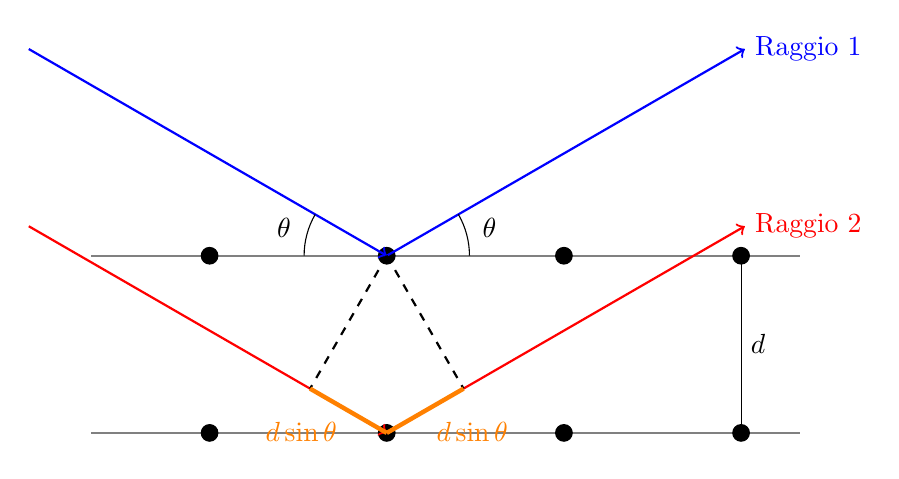
\begin{tikzpicture}[scale=1.5]
    \usetikzlibrary{calc}
    
    % Parametri modificabili a piacimento
    \def\th{30}         % Angolo theta
    \def\d{1.5}         % Distanza interplanare d
    \def\raylen{3.5}    % Lunghezza dei raggi incidenti/riflessi
    
    % Piani
    \draw[thick, gray] (0,0) -- (6,0);
    \draw[thick, gray] (0,-\d) -- (6,-\d);
    \draw[<->] (5.5,0) -- (5.5,-\d) node[midway, right] {$d$};
    
    % Coordinate dei siti reticolari (centri di scattering)
    \coordinate (A) at (2.5, 0);
    \coordinate (B) at (2.5, -\d);
    
    % Atomi
    \foreach \x in {1, 2.5, 4, 5.5} {
        \filldraw[black] (\x,0) circle (2pt);
        \filldraw[black] (\x,-\d) circle (2pt);
    }
    
    % Raggio 1 (Piano superiore)
    % Usa le coordinate polari: da (180-theta) verso A, e da A verso (theta)
    \draw[->, thick, blue] ($(A) + (180-\th:\raylen)$) -- (A);
    \draw[->, thick, blue] (A) -- ($(A) + (\th:\raylen)$) node[right] {Raggio 1};
    
    % Raggio 2 (Piano inferiore)
    \draw[->, thick, red] ($(B) + (180-\th:\raylen)$) -- (B);
    \draw[->, thick, red] (B) -- ($(B) + (\th:\raylen)$) node[right] {Raggio 2};
    
    % Calcolo esatto dei punti C e D per le perpendicolari
    % Si muovono dal punto B lungo la direzione dei raggi per una lunghezza d*sin(theta)
    \coordinate (C) at ($(B) + (180-\th:{\d*sin(\th)})$);
    \coordinate (D) at ($(B) + (\th:{\d*sin(\th)})$);
    
    % Differenza di cammino (perpendicolari tratteggiate)
    \draw[dashed, thick] (A) -- (C);
    \draw[dashed, thick] (A) -- (D);
    
    % Evidenzia la differenza di cammino ottico (ispessimento)
    \draw[ultra thick, orange] (C) -- (B) node[midway, below left] {$d\sin\theta$};
    \draw[ultra thick, orange] (B) -- (D) node[midway, below right] {$d\sin\theta$};
    
    % Archi per gli angoli theta (centrati in A)
    \draw (A) ++(180:0.7) arc (180:180-\th:0.7);
    \node at ($(A) + (180-\th/2:0.9)$) {$\theta$};
    
    \draw (A) ++(0:0.7) arc (0:\th:0.7);
    \node at ($(A) + (\th/2:0.9)$) {$\theta$};
    
\end{tikzpicture}
\end{center}
\vspace{0.5cm}

\subsubsection{Utilizzo della legge di Bragg}

Fissando la lunghezza d'onda $\lambda$, si varia l'angolo $\theta$. Si osservano \textbf{macchie luminose} (bright spots) solo per i valori discreti di $\theta$ che soddisfano la condizione di Bragg per $n = 1, 2, 3, \ldots$. Dalla posizione di queste macchie si ricava la distanza $d$ tra i piani.

Poiché in un cristallo esistono \textbf{infinite famiglie} di piani reticolari (ciascuna con un proprio $d$), il pattern di diffrazione è una collezione di macchie luminose a diversi angoli, corrispondenti alle diverse famiglie. Questo pattern è come un'\textbf{impronta digitale} del cristallo: ogni struttura cristallina produce un pattern unico. Un esperto può identificare il sistema cristallino (cubico, esagonale, ortorombico, ecc.) semplicemente osservando il pattern di diffrazione.

\begin{nota}
Anche se le famiglie di piani sono infinite, la condizione $2d\sin\theta = n\lambda$ seleziona solo un \textbf{insieme discreto} di angoli $\theta$, e questo insieme è unico per ogni cristallo.
\end{nota}

\subsubsection{Limiti della formulazione di Bragg e anticipazione di Von Laue}

Nella formulazione di Bragg, si \textbf{assume} l'esistenza dei piani reticolari come punto di partenza. Una domanda legittima è: perché i piani reticolari dovrebbero esistere? Sono reali o solo una costruzione mentale?

Nella prossima lezione si presenterà la \textbf{formulazione di Von Laue}, che:
\begin{itemize}
    \item \textbf{Non assume} l'esistenza dei piani reticolari.
    \item Formula lo scattering in modo indipendente.
    \item Il risultato coincide con la legge di Bragg, facendo \textbf{emergere} i piani reticolari come conseguenza.
\end{itemize}

Questo conferma che Bragg ebbe un'intuizione eccellente, anche se la sua assunzione iniziale non era giustificata a priori.

\section{Nota: reticolo reciproco di un reticolo con base}

\textbf{Domanda:} è possibile definire il reticolo reciproco di un reticolo di Bravais con base?\\
\textbf{Risposta:} il concetto di reticolo reciproco è definito \textbf{solo} per il reticolo di Bravais sottostante. La base \textbf{non interviene} nella definizione del reticolo reciproco.

Ad esempio, per il reticolo a nido d'ape (honeycomb), che è un reticolo esagonale con base di 2 atomi, il reticolo reciproco è semplicemente il reticolo reciproco del \textbf{reticolo esagonale}. La base non compare nello spazio reciproco.


\textbf{Domanda naturale}: allora come si distingue, tramite scattering X, un reticolo puro da un reticolo con base? Questa distinzione è possibile e verrà trattata nelle lezioni successive. La base introduce effetti nello scattering (il cosiddetto \textbf{fattore di forma}), ma il reticolo reciproco in sé rimane quello del reticolo di Bravais fondamentale.
